\chapter{About}\label{ch:about}

% CONTENT
% about book
% - how did it all start? initial intention/motivation?
% - what is the goal of this book? who is the target group? what different after book read?
% about me
% - to underestand psycho-analysis, understand freud; sociocultural environment, the time he lived (child of his time)
% - my background, thus my approaches/opinions/biases (not to show-off ego thing)
% - pragmatic approach; technical, "manly", less aesthetics; functional (martial arts)

\begin{figure}[h]
    \begin{center}
      \makebox[\textwidth]{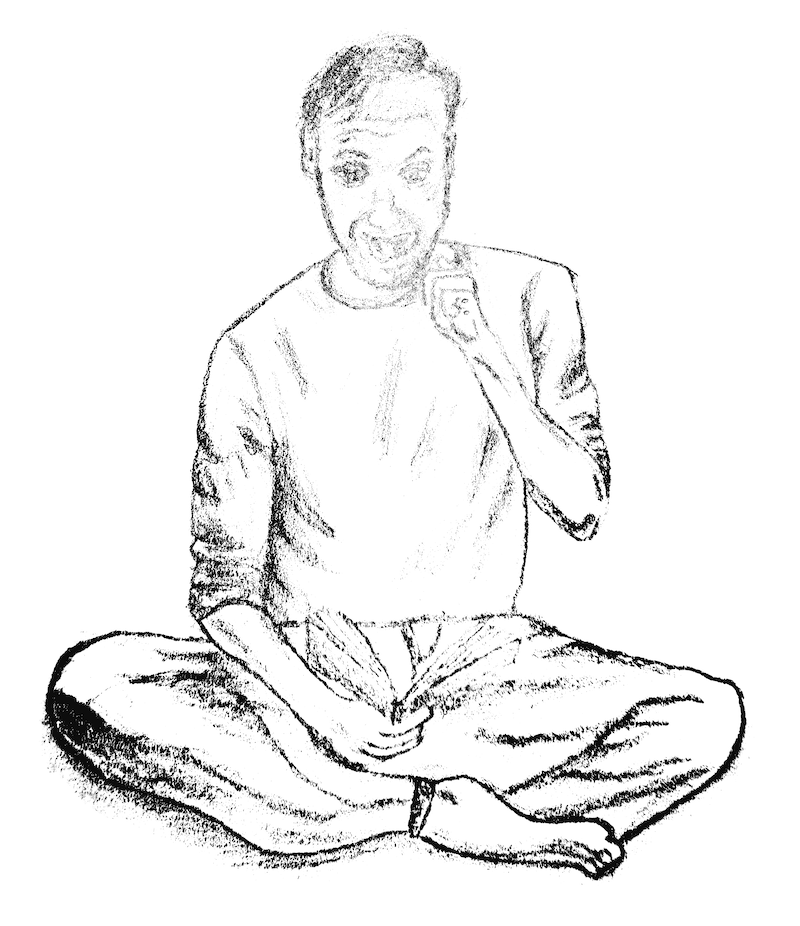
\includegraphics[width=0.3\paperwidth]{images/testpic}}
    \end{center}\label{fig:testpic}
\end{figure}

%\begin{wrapfigure}{R}{0.3\textwidth}
%\centering
%\includegraphics[width=0.25\textwidth]{images/about}
%\end{wrapfigure}

So what is this book about, and who has written it?
For whom is it written, and where is its emphasis?
And also some general remarks as a form of a disclaimer before continue reading.

\section{Book}\label{sec:book}

The following pages were initially written for the sole purpose of taking \textbf{personal notes}, but then it started to grow further and further, and now it reached a level where it could also be of use to others; whether to those which consider themselves \textbf{beginners or more experienced} practitioners.
Everyone who is interested in getting more acquainted with the \textbf{theoretical background} -- next to their regular practice in the dance studio -- of the fine art of Contact Improvisation Dance, or simply \textbf{CI} for short as of now, may find something useful in this book.

Whatever is written here does not claim to hold any absolute, objective truth, but merely is a manifestation of a very \textbf{personal, subjective} collection of experiences, thoughts, observations and opinions which were gathered along a single person's journey.
It also holds no claim whatsoever to be complete in any way, as any form of completeness can never be achieved any way, as we are not dealing with a hard science here; so be gentle when you encounter an attempt of enumerating possibilities which you know is missing something.
If you do so, please consider contacting me, contributing to this little project, and bringing it closer to completion and perfection, yet knowing we will never reach it, an asymptotic goal.
Some parts are summaries of sources found along a path of exploration, whether they might be (direct or indirect) oral teachings, or written information found in books or on the internet.
The content is, of course, also \textbf{partially biased}, although the best attempts were made to free oneself from one's own limitations of perception of reality, and thus, the content will sometimes be colored by a personal background -- I shall be forgiven for my flawed human nature.

The book uses the \textbf{masculine version} when using examples for the sake of simplicity, in case both can be applied, and of course, always implying that the female version could have been equally used as well.

\section{Myself}\label{sec:myself}

My background lies mainly with internal \textbf{Martial Arts}, and as such, my focus lies more on a practical approach (``\textit{Good Kung-Fu looks bad, only bad Kung-Fu looks good!}''), where ``\textit{form follows function}'', and less about the aesthetics of movement which might be more important to a dancer.
``Right'' is what works in the \textbf{most pragmatic} way, meaning efficient in time and space (physics/biomechanics), and as well whatever is within principles of CI.

Besides those more physical aspects, the \textbf{psychological aspect} also has an important role to me: The benefit for one's mental health, the ability to get to know oneself and others more deeply, and of course a more philosophical/spiritual path which can also be walked with the help of this deep art.

Also, as a body worker, I emphasize the importance of the non-verbal communication aspect of movement between two people.
The slowness, the gentleness in establishing a \textbf{deep connection} through listening, and the expressions of our personalities through this practice.
